\documentclass[
  manuscript=report,  %% article (default), rescience, data, or software
  layout=preprint,  %% preprint (for submission) or publish (for publisher only)
  year=20xx,
  volume=x,
]{extra/joas}

%\doi{10.74800/joas.x.xxxx}


%\received {1 April 2022}
%\revised  {1 May 2022}
%\accepted {10 May 2022}
%\published{20 May 2022}
%\editor{Editor Name}
%\reviewers{First Reviewer, Second Reviewer, Third Reviewer}


% --- blew is the area for authors ---

\usepackage{float}
\usepackage[english]{babel}
\usepackage{blindtext}

% specify the .bib file for references
\usepackage{biblatex}
\addbibresource{reference.bib} 

% Make sure your article tile is within 12 words
\title{Predictive Maintainance using Deep Learning}


%\email{correspondence@email.domain}

\author{Giriraj Pawar}
\affiliation{FusionSystems GmbH, Chemnitz}

\author{Michael Kaiser}
\affiliation{FusionSystems GmbH, Chemnitz}

\author{Karsten Schwalbe}
\affiliation{FusionSystems GmbH, Chemnitz}

\author{Daniel Lohmeier-von Laer}
\affiliation{FusionSystems GmbH, Chemnitz}




%\author{Third Author}
%\alsoaffiliation{Institution-1, City, Country}
%\affiliation{Institution-3, City, Country}


% maximum five keywords
\keywords{} 

% Important, only index abbreviation if a term contains more than two words, and the term is used more than ten times throughout the paper. Otherwise, spell them out in full in the paper.
\abbreviations{}


\begin{document}

%\begin{abstract}
%  
%\end{abstract}


\section{Introduction}

In the era of Industry 4.0, sensors are installed on machinery for real-time data collection, processing, and automation. The collected data availed to build deep learning models for predictive maintenance and condition monitoring. One such sensor is the vibration sensor. They are used to detect several abnormalities in industrial machinery. In this task, a test setup is constructed, which simulates an industrial machine, and the data is collected using a vibration sensor installed upon it. Further, the collected data processed and benefited to build deep learning models and conduct investigations associated with the estimation of speed of rotors and rotating unbalance.

%\blindtext 
%Some example open open-source research data \cite{schafer2014bringing} and tools \cite{olive2019traffic}. 


%\blindtext [2]


%\section{Literature Survey}

%\section{Setup}


%\subsection{Dataset Creation}


\section{Method}

The FCN (Fully Convolutional Network) has been a state-of-the-art solution for semantic segmentation, image classification, and object detection. Over the years, it has attained compelling results and acts as an efficient feature extractor\cite{https://doi.org/10.48550/arxiv.1411.4038}. Nowadays, for predictive maintenance and condition monitoring tasks, FCN is used broadly. In this task, the classification models are constructed using FCN. The proposed model architecture mainly has three blocks. Each block has a 1D convolution layer followed by batch normalization and ReLU activation layers. The batch normalization layer helps in improving training speed and generalization. Each convolution block has 64 filters and the convolution is performed by a 1D kernel of size 5. After these three blocks, features are fed to the global average pooling layer, which reduces the number of learnable parameters. Next, its output is passed through the softmax layer to obtain final labels. The architecture of the model is illustrated in figure \ref{fig:FCN}.

\begin{equation} \label{eq:FCN}
\begin{aligned}
y = W \circledast x + b\\
s = BN(y)\\
h = ReLU(s)
\end{aligned}
\end{equation}

%\vspace*{0.5cm}

%\footnote{Detailed information about the \href{https://scikit-learn.org/stable/modules/generated/sklearn.preprocessing.StandardScaler.html}{StandardScalar} preprocessing method provided in scikit-learn documentation (last access 20.03.2023).}

The time series data collected from the vibration sensor is 3D. Initially, the data is preprocessed using the StandardScaler method\footnote{Scikit-learn documentation provides detailed information about the \href{https://scikit-learn.org/stable/modules/generated/sklearn.preprocessing.StandardScaler.html}{StandardScalar} preprocessing method (Last accessed on 20.03.2023).} and fed to the model for training. The StandardScaler standardizes features by subtracting the mean and scaling to unit variance. The standard score $z$ of a sample $x$ is calculated using equation \ref{eq:StandardScalar}, where $\mu$ is the mean and $s$ is the standard deviation.

%\vspace*{0.5cm}
\begin{equation} \label{eq:StandardScalar}
z = \frac{(x - \mu)}{s}
\end{equation}

The ADAM\cite{kingma2017adam} optimization algorithm is used to train the model, with an initial learning rate of 0.001. The sparse categorical crossentropy loss function is used to compute the training and validation loss. Later, the model is evaluated by sparse categorical accuracy metric during training, validation, and testing. TensorBoard\footnote{\href{https://www.tensorflow.org/tensorboard}{TensorBoard} is TensorFlow's visualization toolkit for machine learning experiments (Last accessed on 24.03.2023).} is used to observe the loss and accuracy metrics during training and validation at each epoch. Keras callbacks are used for early stopping, to reduce the learning rate, and to save the best model using monitored quantity, such as validation loss. It is recommended to use tf. data APIs from Tensorflow to construct the input pipeline, as they are efficient and don't overflow the memory.

\begin{figure}[ht!]
  \centering
  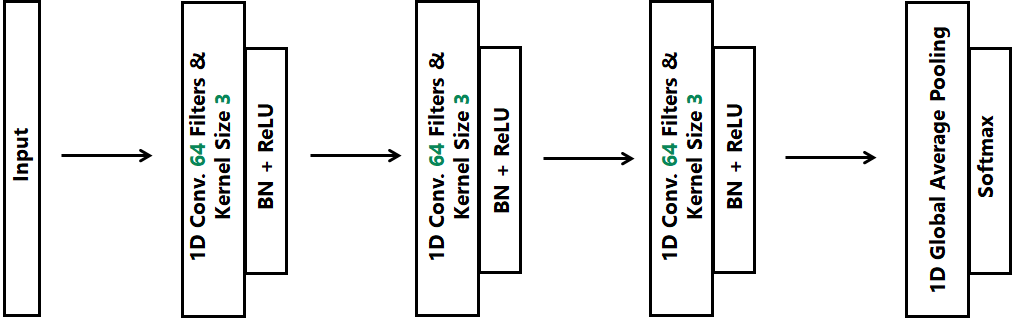
\includegraphics[width=0.8\textwidth]{figures/FCN.png}
  \caption{Architecture of the model using FCN for time series classification.}
  \label{fig:FCN}
\end{figure}


%\paragraph{Paragraph title} This is the paragraph with title if you want to use such function in the paper. This is the paragraph with title if you want to use such function in the paper
%This is the paragraph with title if you want to use such function in the pape %\blindtext


\section{Experiments}

This section describes experiments that were carried out and their outcomes. In the first experiment, the data collected by attaching distinct rotating unbalance is used to train a classification model. In the second experiment, another classification model is trained using the data collected at different speeds. 

%The test setup constructed for data collection is displayed in the figure \ref{fig:diVibestestSetup}.

%
%\begin{figure}[ht!]
%  \centering
%  \begin{minipage}[b]{0.48\textwidth}
%    \includegraphics[width=\textwidth]{figures/testSetup1.png}
%    \caption{diVibes test setup. (a) The placement of the Vibration Sensor. (b) A rotating unbalance is attached to a rotar.}
%    \label{fig:diVibestestSetup}
%  \end{minipage}
%%  \hfill
%  \begin{minipage}[b]{0.48\textwidth}
%    \includegraphics[width=\textwidth]{figures/testSetup2.png}
%  \end{minipage} 
%\end{figure}

\subsection{Estimation of the Rotating Unbalance}

One of the main reasons for vibrations in industrial machinery is the rotating unbalance. If these machines are not maintained, the unbalance causes high vibrations, noise, and ultimately failure of the complete system which creates a hazardous environment inside the industrial plant. In this experiment, a classification model is trained using time series data collected using a vibration sensor placed near the rotor, to which four unbalances of distinct weight are attached. The unbalances are A1 (Aluminum block of 22.35 gms), A2 (Aluminum block of 23.05 gms), A1+A2 (Combined two Aluminum blocks A1 and A2 weighing 45.40 gms in total), and S1 (Steel block of 30.50 gms). The trained Rotating Unbalance Classifier is an optimal fit as learning curves of training and validation losses both decrease and stabilize, as shown in figure \ref{fig:trainingAndValidationLossAccuracy}. On the test dataset, the model is 99.16\% accurate. Test results are illustrated by plotting a confusion matrix shown in figure \ref{fig:rotatingUnbalanceCM}.


The trained Rotating Unbalance Classifier is generalized well and optimally fit as learning curves of training and validation losses both decrease and stabilize, shown in figure \ref{fig:trainingAndValidationLossAccuracy}.
 

\begin{figure}[ht!]
  \centering
  \begin{minipage}[b]{0.48\textwidth}
    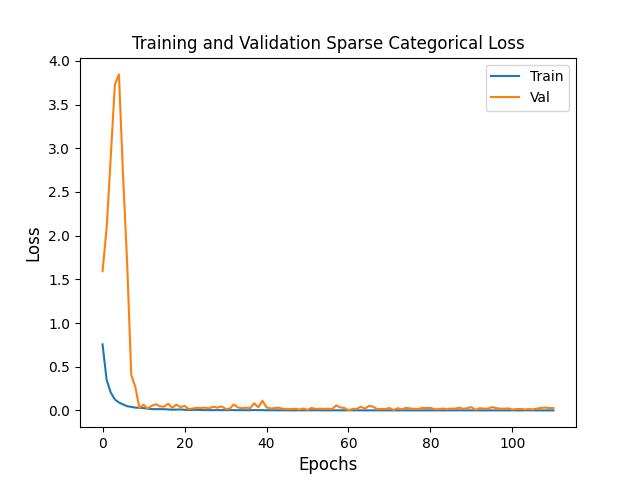
\includegraphics[width=\textwidth]{figures/trainingAndValidationLoss.png}
    \caption{Training and validation learning curves while training Rotating Unbalance Classifier.}
    \label{fig:trainingAndValidationLossAccuracy}
  \end{minipage}
%  \hfill
  \begin{minipage}[b]{0.48\textwidth}
    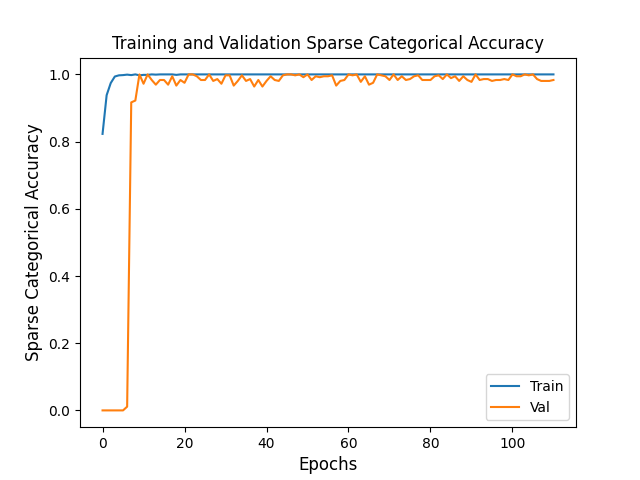
\includegraphics[width=\textwidth]{figures/trainingAndValidationAccuracy.png}
    %\caption{Training and validation accuracy during the training.}
  \end{minipage} 
\end{figure}

\begin{figure}[ht!]
  \centering
  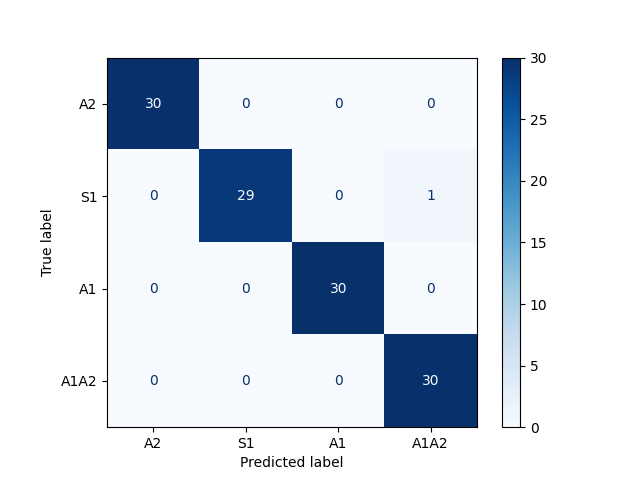
\includegraphics[width=0.6\textwidth]{figures/confusionMatrix.png}
  \caption{Illustration of the performance of the Rotating Unbalance Classifier on the test dataset using a confusion matrix.}
  \label{fig:rotatingUnbalanceCM}
\end{figure}


\subsection{Estimation of the Speed}

Speed estimation is one of the vital tasks in condition monitoring to determine the status of industrial machines. Bearing faults, aging spare parts, electrical failures, and other anomalies can decrease the speed of rotors. In this experiment, a classification model is trained using time series data collected at distinct speeds, such as 600 RPM, 800 RMP, 1000 RPM, and 1200 RPM, with block of Rotating Unbalance A1 attached to the rotor. The trained Speed Classifier is an optimal fit as learning curves of training and validation losses both decrease and stabilize, shown in figure \ref{fig:speedClassifierTrainingAndValidationLossAccuracy}. On the test dataset, the model is 100\% accurate. Test results are illustrated by plotting a confusion matrix shown in figure  \ref{fig:speedClassifierCM}.



\begin{figure}[ht!]
  \centering
  \begin{minipage}[b]{0.48\textwidth}
    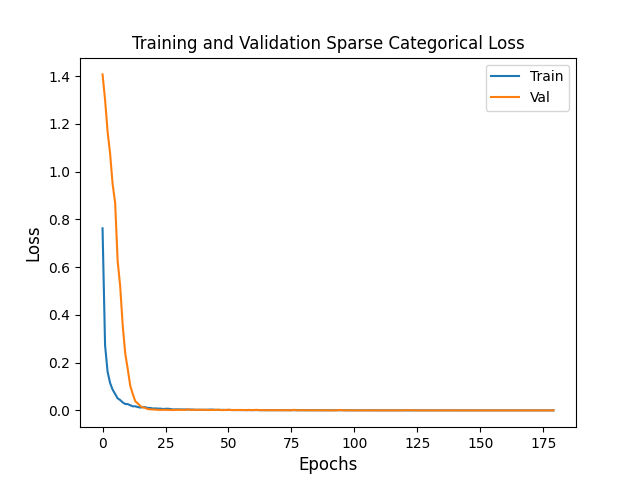
\includegraphics[width=\textwidth]{figures/speedClassifierTrainingAndValidationLoss.png}
    \caption{Training and validation learning curves while training Speed Classifier.}
    \label{fig:speedClassifierTrainingAndValidationLossAccuracy}
  \end{minipage}
%  \hfill
  \begin{minipage}[b]{0.48\textwidth}
    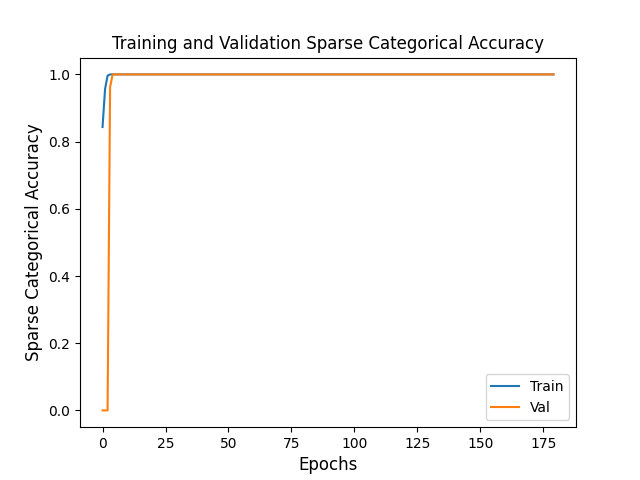
\includegraphics[width=\textwidth]{figures/speedClassifierTrainingAndValidationAccuracy.png}
    %\caption{Training and validation accuracy during the training.}
  \end{minipage}
\end{figure}


\begin{figure}[ht!]
  \centering
  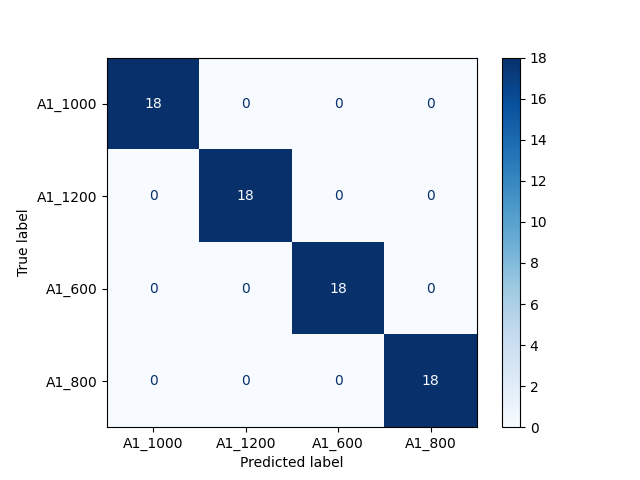
\includegraphics[width=0.6\textwidth]{figures/speedClassifierConfusionMatrix.png}
  \caption{Illustration of the performance of the Speed Classifier on the test dataset using a confusion matrix.}
  \label{fig:speedClassifierCM}
\end{figure}

%\blindtext The end result is in Figure \ref{fig:logo}.

%\begin{figure}[ht!]
%  \centering
%  
\includegraphics[width=0.6\textwidth]{figures/joas-logo.pdf}
%  \caption{JOAS Logo}
%  \label{fig:logo}
%\end{figure}

%\blindtext\footnote{This is how a footnote works.}

%\subsection{Method}

%\subsubsection{Method part 2-1}

%\blindtext Reference to Equation \ref{eq:cauchy_momentum}.
%
%\begin{equation} \label{eq:cauchy_momentum}
%\rho\frac{\mathrm{D} \mathbf{u}}{\mathrm{D} t} = - \nabla p + \nabla \cdot \boldsymbol \tau + \rho\,\mathbf{g}
%\end{equation}


%\subsubsection{Method part 2-2}

%\blindtext Table \ref{tb:example_table} shows an example.

%\begin{table}[H]
%  \centering
%  \small
%  \caption{Example table}
%  \label{tb:example_table}
%  \begin{tabular}{lll}
%  \toprule
%  \textbf{Parameter} & \textbf{Notation} & \textbf{Remarks} \\
%  \midrule
%  name & - & engine common identifier \\
%  manufacture & - & name of the manufacture  \\
%  bpr & $\lambda$ & bypass ratio \\
%  pr & - & pressure ratio \\
%  thrust & $T_0$ & maximum static thrust\\
%  \bottomrule
%  \end{tabular}
%\end{table}

%\blindtext


%\section{Discussions}
%
%\paragraph{Paragraph title} This is the paragraph with title if you want to use such function in the paper. \blindtext


\section{Conclusion}

The primary goal of this task is to draft a proof-of-concept for predictive maintenance and condition monitoring of industrial machines using deep learning models. Therefore, a test setup simulating an industrial machine is constructed. Later, classification models are trained using the time series data collected from the vibration sensor installed upon it. The investigations reveal that the trained Rotating Unbalance Classifier and Speed Classifier are almost 100\% accurate on unseen test data.

%\blindtext

%\appendix
%
%\section{Supplementary figures}
%\blindtext
%
%\section{Supplementary tables}
%\blindtext
%
%
%\begin{acknowledgement}
%  Include your acknowledgement in this section.
%\end{acknowledgement}
%
%% Author contributions (CRediT) are mandatory for all papers with more than one author
%\begin{credit}
%  If the paper has more than one author, the CRediT section must be included. See example usage on \url{https://casrai.org/credit/}
%
%  \begin{itemize}
%    \item First Author: Conceptualization, Methodology, Software, Writing- Original draft
%    \item Second Author: Data curation, Writing- Original draft
%    \item Third Author: Visualization, Investigation
%  \end{itemize}
%\end{credit}


%\begin{funding}
%  When applicable, please specify the funding information for this research.
%\end{funding}


% Data statement is mandatory for all papers
%\begin{opendata}
%  DOI and short description to supplementary data.
%\end{opendata}

% reproducibility statement is mandatory for all papers
%\begin{reproduce}
%Information on how to reproduce this research, including access to 1) source code related the research, 2) source code for the figures, 3) source code / data for the tables when applicable.
%\end{reproduce}



\newpage
\printbibliography



\end{document}
